%Description des fonctions à servir (diagramme des cas d'utilisation)

\subsection{Cadre de travail}
La quantité de documents non organisés de la prefecture de Mayenne est considérable.
Aussi, réaliser un système permettant de traiter tous ces documents, de styles et de types très différents, n'était pas réalisable dans les 6 mois alloués au projet.
Nous et le commanditaire avons donc convenu de la réalisation d'un \textit{Proof Of Concept} se focalisant uniquement sur les documents de type `Recueil des Actes Administratifs' (RAA).
Ces documents sont publiés publiquement au moins une fois par mois, et contiennent tous les actes à caractère réglementaire non personnels publiés durant le mois dernier.
Certains RAA qualifiés de \textit{spéciaux} peuvent également être publiés à titre exceptionnel durant le mois.
On observe en moyenne 130 RAA publiés par an.

Dans le cadre du projet, nous avons récupéré tous les RAA de l'année 2016 à 2019, c'est a dire 431 documents.
Chaque RAA regroupe plusieurs arrêtés pouvant traiter de sujets très divers, de l'interdiction de manifestation à la délégation de signature.

Le cadre d'étude du projet est donc très large mais suffisamment restreint pour qu'il soit possible de produire un POC dans les délais impartis. 

\begin{figure}[h!]
  \centering
  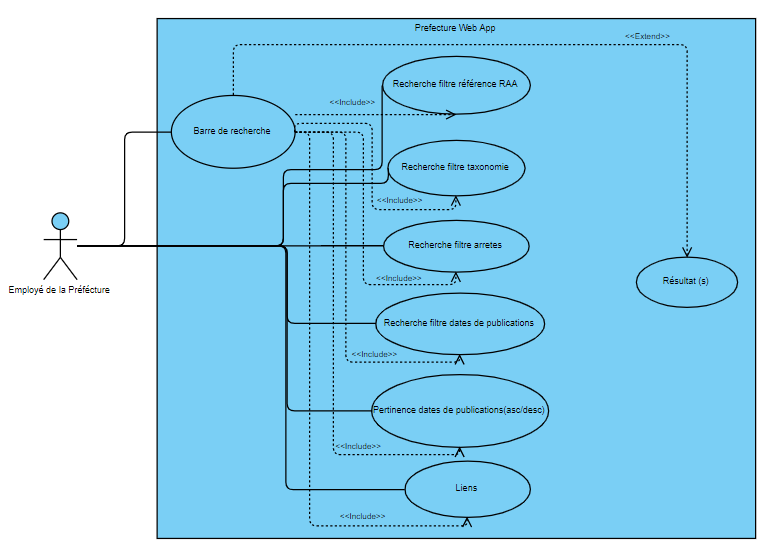
\includegraphics[width=0.7\textwidth]{uml_utilisation.png}
	\caption[]{Diagramme UML des cas d'utilisation}
	\label{fig:umlUtilisation}
\end{figure}

Pour notre commanditaire, il est également essentiel que l'ensemble du projet et les outils utilisés soient open source.
Cette contrainte a été respectée tout au long du projet, et nous n'avons donc pas jugé utile de préciser que tous les outils présentés sont open source.

\subsection{Extraction du texte brut}
Tous les RAA récents sont disponibles en ligne en version PDF, ce qui leur permet d'être accessibles facilement par n'importe qui sur le site de la prefecture.
Nous avons besoin de récupérer le texte brut (appelé transcript) des documents afin d'en extraire les informations d'importance.

Généralement, le format PDF contient le texte brut du document afin d'en réduire le poids de stockage, une image nécessitant plus de mémoire que du simple texte.
Malheureusement certains RAA ont d'abord été imprimés pour être signés, puis scannés pour leur mise en ligne.
Les documents ainsi scannés ne contiennent pas le texte brut, et récupérer le transcript est bien plus complexe.


\subsection{Recherche d'informations d'importance}\label{infosImp}
Chaque document contient des informations d'importance qui doivent être extraites pour que le document en question soit correctement classé par la suite.
Les informations d'importance, déterminées avec le commanditaire, sont les suivantes:
\begin{itemize}
\item Référence du RAA
\item Nom du signataire
\item Date de publication
\item Dates mentionnées
\item Références des arrêtés
\item Titre des arrêtés
\item Références des décrets
\item Références des articles
\item Références des lois
\item Noms des parties prenantes
\item Lieux mentionnés
\item Noms d'organisation et d'organismes
\end{itemize}

Ces éléments sont les plus susceptibles d'être utilisés lors de la recherche par un utilisateur de notre POC et sont également les plus pertinents pour la classification.



\subsection{Classement par taxonomie}
Une taxonomie est un ensemble fermé de termes organisés sous la forme d'un arbre permettant de \textit{tagger} précisément un document en fonction de son contenu afin de normaliser sa classification (Voir figure~\ref{fig:tree}).
L'utilisation d'une taxonomie permet de regrouper les documents selon des critères objectifs et standards, indépendants de la méthode de classification individuelle utilisée par les employés de la prefecture.
L'administration Française a établi plusieurs taxonomies en fonction des services (archives, \ldots).
L'inconvénient de la taxonomie est sa taille importante: il est impossible de connaitre parfaitement l'ensemble de l'arbre et donc par conséquent, le classement taxonomique d'un document par un humain est probablement incomplet, incorrect, voir le plus souvent totalement absent.

Pour le commanditaire, il est essentiel que nous ajoutions une taxonomie au document.
Il nous a donc fourni une taxonomie réduite de plus de 6000 termes.


\subsection{Moteur de recherche}
Afin de montrer l'utilité des informations extraites des documents, nous devons également réaliser un moteur de recherche basique.
Ce moteur de recherche a deux utilisations principales: 
\begin{itemize}
\item \textbf{Suggestions de recherche}:\newline
Afin de retrouver des documents, nous devons mettre en place un système de recherche intelligente.
Ce système agira comme une barre de recherche google, en proposant des résultats pertinents, tout en mettant à disposition des filtres pour affiner les recherches.

\item \textbf{Apparence}:\newline
Le moteur de recherche permettra aussi à notre commanditaire de présenter le projet à la prefecture devant un public.
Donner une apparence simple à un projet complexe est une tâche très importante pour des clients qui recherchent justement la simplicité.
\end{itemize}

